% Copyright (C) Rosita Wachenchauzer <rositaw@gmail.com>

% Esta obra está licenciada de forma dual, bajo las licencias Creative
% Commons:
%  * Atribución-Compartir Obras Derivadas Igual 2.5 Argentina
%    http://creativecommons.org/licenses/by-sa/2.5/ar/
%  * Atribución-Compartir Obras Derivadas Igual 3.0 Unported
%    http://creativecommons.org/licenses/by-sa/3.0/deed.es_AR.
%
% A su criterio, puede utilizar una u otra licencia, o las dos.
% Para ver una copia de las licencias, puede visitar los sitios
% mencionados, o enviar una carta a Creative Commons,
% 171 Second Street, Suite 300, San Francisco, California, 94105, USA.

\chapter[Conceptos básicos]{Algunos conceptos básicos}

En esta unidad hablaremos de lo que es un programa de
computadora e introduciremos unos cuantos conceptos referidos a la
programación y a la ejecución de programas. Utilizaremos en todo
momento el lenguaje de programación Python para ilustrar esos
conceptos.

\section{Computadoras y programas}

En la actualidad, la mayoría de nosotros utilizamos computadoras
permanentemente: para mandar correos electrónicos, navegar por Internet,
chatear, jugar, escribir textos.

Las computadoras se usan para actividades tan disímiles como predecir las
condiciones meteorológicas de la próxima semana, guardar historias clínicas,
diseñar aviones, llevar la contabilidad de las empresas o controlar una
fábrica. Y lo interesante aquí (y lo que hace apasionante a esta carrera) es
que el mismo aparato sirve para realizar todas estas actividades: uno no
cambia de computadora cuando se cansa de chatear y quiere jugar al solitario.

Muchos definen una computadora moderna como ``una máquina que
almacena y manipula información bajo el control de un programa que
puede cambiar''. Aparecen acá dos conceptos que son claves: por un
lado se habla de una {\it máquina} que almacena información, y por
el otro lado, esta máquina está controlada por {\it un programa
que puede cambiar}.

Una calculadora sencilla, de esas que sólo tienen 10 teclas para
los dígitos, una tecla para cada una de las 4 operaciones, un
signo igual, encendido y CLEAR, también es una máquina que
almacena información y que está controlada por un programa. Pero
lo que diferencia a esta calculadora de una computadora es que en
la calculadora el programa no puede cambiar.

Un {\it programa de computadora} es un conjunto de {\it
instrucciones} paso a paso que le indican a una computadora cómo
realizar una tarea dada, y en cada momento uno puede elegir
ejecutar un programa de acuerdo a la tarea que quiere realizar.

Las instrucciones se deben escribir en un lenguaje que nuestra
computadora entienda. Los lenguajes de programación son
lenguajes diseñados especialmente para dar
órdenes a una computadora, de manera exacta y no ambigua. Sería
muy agradable poder darle las órdenes a la computadora en
castellano, pero el problema del castellano, y de las lenguas
habladas en general, es su ambigüedad:

Si alguien nos dice {\it ``Comprá el collar sin monedas''}, no sabremos
si nos pide que compremos el collar que no tiene monedas, o que compremos
un collar y que no usemos monedas para la compra. Habrá que preguntarle
a quien nos da la orden cuál es la interpretación correcta. Pero tales
dudas no pueden aparecer cuando se le dan órdenes a una computadora.

Este curso va a tratar precisamente de cómo se escriben programas
para hacer que una computadora realice una determinada tarea.
Vamos a usar un lenguaje específico (Python) porque es sencillo y
elegante, pero éste no será un curso de Python sino un curso de
programación.

\begin{sabias_que}
Existe una gran cantidad de programas desarrollados en Python, desde
herramientas para servidores, como {\bf mailman}, hasta programas amigables
para usuarios finales, como {\bf emesene}, pasando por aplicaciones
empresariales, {\bf openerp}, {\bf tryton}; herramientas de desarrollo,
{\bf meld}, {\bf mercurial}, {\bf bazaar}, {\bf trac}; plataformas web,
{\bf django}, {\bf turbogears}, {\bf zope}; clientes de bittorrent, {\bf
bittorrent}, {\bf bittornado}, {\bf deluge}; montones de juegos de todo
tipo, y muchísimas aplicaciones más.

Todas estas aplicaciones son software libre, por lo que se puede obtener y
estudiar el código con el que están hechas
\end{sabias_que}

\section{El mito de la máquina todopoderosa}

Muchas veces la gente se imagina que con la computadora se puede
hacer cualquier cosa, que no hay tareas imposibles de realizar.
Más aún, se imaginan que si bien hubo cosas que eran imposibles de
realizar hace 50 años, ya no lo son más, o no lo serán dentro de
algunos años, cuando las computadoras crezcan en poder (memoria,
velocidad), y la computadora se vuelva una máquina todopoderosa.

Sin embargo eso no es así: existen algunos problemas, llamados
{\it no computables} que nunca podrán ser resueltos por una
computadora digital, por más poderosa que ésta sea. La
computabilidad es la rama de la computación que se ocupa de
estudiar qué tareas son computables y qué tareas no lo son.

De la mano del mito anterior, viene el mito del lenguaje
todopoderoso: hay problemas que son no computables porque en
realidad se utiliza algún lenguaje que no es el apropiado.

En realidad todas las computadoras pueden resolver los mismos
problemas, y eso es independiente del lenguaje de programación que
se use. Las soluciones a los problemas computables se pueden
escribir en cualquier lenguaje de programación. Eso no significa
que no haya lenguajes más adecuados que otros para la resolución
de determinados problemas, pero la adecuación está relacionada con
temas tales como la elegancia, la velocidad, la facilidad para
describir un problema de manera simple, etc., nunca con la
capacidad de resolución.

Los problemas no computables no son los únicos escollos que se le
presentan a la computación. Hay otros problemas que si bien son
computables demandan para su resolución un esfuerzo enorme en
tiempo y en memoria. Estos problemas se llaman {\it intratables}.
El análisis de algoritmos se ocupa de separar los problemas
tratables de los intratables, encontrar la solución más barata
para resolver un problema dado, y en el caso de los intratables,
resolverlos de manera aproximada: no encontramos la verdadera
solución porque no nos alcanzan los recursos para eso, pero
encontramos una solución bastante buena y que nos insume muchos
menos recursos (el orden de las respuestas de Google a una
búsqueda es un buen ejemplo de una solución aproximada pero no
necesariamente óptima).

En este curso trabajaremos con problemas no sólo computables sino
también tratables. Y aprenderemos a medir los recursos que nos
demanda una solución, y empezaremos a buscar la solución menos
demandante en cada caso particular. \\

Algunos ejemplos de los problemas que encararemos y de sus
soluciones:

\begin{problemac}
Dado un número $N$ se quiere calcular $N^{33}$.
\end{problemac}

Una solución posible, por supuesto, es hacer el producto $N \times
N \times \ldots \times N$, que involucra 32 multiplicaciones.

Otra solución, mucho más eficiente es:
\begin{itemize}
\item Calcular $N \times N$.

\item Al resultado anterior mutiplicarlo por sí mismo con lo cual
ya disponemos de $N^{4}$.

\item Al resultado anterior mutiplicarlo por sí mismo con lo cual
ya disponemos de $N^{8}$.

\item Al resultado anterior mutiplicarlo por sí mismo con lo cual
ya disponemos de $N^{16}$.

\item Al resultado anterior mutiplicarlo por sí mismo con lo cual
ya disponemos de $N^{32}$.

\item Al resultado anterior mutiplicarlo por $N$ con lo cual
conseguimos el resultado deseado con sólo 6 multiplicaciones.

\end{itemize}

Cada una de estas dos soluciones representa un {\it algoritmo}, es
decir un método de cálculo, diferente. Para un mismo problema
puede haber algoritmos diferentes que lo resuelven, cada uno con
un costo distinto en términos de recursos computacionales
involucrados.

\begin{sabias_que}
La palabra \textit{algoritmo} no es una variación de \textit{logaritmo},
sino que proviene de \textit{algorismo}. En la antigüedad, los
\textit{algoristas} eran los que calculaban usando la numeración arábiga y
mientras que los \textit{abacistas} eran los que calculaban usando ábacos.
Con el tiempo el \textit{algorismo} se deformó en \textit{algoritmo},
influenciado por el término \textit{aritmética}.

A su vez, el uso de la palabra \textit{algorismo} proviene del nombre de un
matemático persa famoso, en su época y para los estudiosos de esa época,
``Abu Abdallah Muhammad ibn Mûsâ al-Jwârizmî'', que literalmente significa:
``Padre de Ja'far Mohammed, hijo de Moises, nativo de Jiva''. Al-Juarismi,
como se lo llama usualmente, escribió en el año 825 el libro ``Al-Kitâb
al-mukhtasar fî hîsâb al-gabr wa'l-muqâbala'' (Compendio del cálculo por el
método de completado y balanceado), del cual surgió también la palabra
``álgebra''.

Hasta hace no mucho tiempo se utilizaba el término algoritmo para referirse
únicamente a formas de realizar ciertos cálculos, pero con el surgimiento
de la computación, el término algoritmo pasó a abarcar cualquier método
para obtener un resultado.
\end{sabias_que}

\begin{problemac}

Tenemos que permitir la actualización y consulta de una guía
telefónica.

\end{problemac}

Para este problema no hay una solución única: hay muchas y cada
una está relacionada con un contexto de uso. ¿De qué guía estamos
hablando: la guía de una pequeña oficina, un pequeño pueblo, una
gran ciudad, la guía de la Argentina? Y en cada caso ¿de qué tipo
de consulta estamos hablando: hay que imprimir un listado una vez
por mes con la guía completa, se trata de una consulta en línea,
etc.? Para cada contexto hay una solución diferente, con los datos
guardados en una {\it estructura de datos} apropiada, y con
diferentes algoritmos para la actualización y la consulta.

%
% TODO: incluir aunque sea un esbozo de la solución a este problema
%

\section{Cómo darle instrucciones a la máquina usando Python}

\begin{sabias_que}
Python fue creado a finales de los años 80, por un programador holandés
llamado Guido van Rossum, quien sigue siendo aún hoy el líder del
desarrollo del lenguaje.

La versión 2.0, lanzada en 2000, fue un paso muy importante para el
lenguaje ya que era mucho más madura, incluyendo un \textit{recolector de
basura}.  La versión 2.2, lanzada en diciembre de 2001, fue también un hito
importante ya que mejoró la orientación a objetos.  La última versión de
esta línea es la 2.7 que fue lanzada en noviembre de 2010 y aún está vigente.

En diciembre de 2008 se lanzó la rama 3.0, cuya versión actual es la 3.5, de
septiembre de 2015, y es la que utilizamos en este libro. Python 3 fue diseñado
para corregir algunos defectos de diseño en el lenguaje, y muchos de los
cambios introducidos son incompatibles con las versiones anteriores. Por esta
razón, las ramas 2.x y 3.x coexisten con distintos grados de adopción.
\end{sabias_que}

El lenguaje Python nos provee de un {\it intérprete}, es decir un programa que
interpreta las órdenes que le damos a medida que las escribimos. La forma más
típica de invocar al intérprete es ejecutar el comando |python3| en
la terminal.

\begin{atencion}
De forma tal de aprovechar al máximo este libro, recomendamos instalar Python 3
en una computadora, y acompañar la lectura probando todos los ejemplos de
código y haciendo los ejercicios.

En \url{https://www.python.org/downloads/} se encuentran los enlaces para
descargar Python, y en
\url{http://docs.python.org.ar/tutorial/3/interpreter.html} hay más información
acerca de cómo ejecutar el intérprete en cada sistema operativo.
\end{atencion}

\begin{lstlisting}[language={},numbers=none]
$ python3
Python 3.5.0 (default, Sep 20 2015, 11:28:25)
[GCC 5.2.0] on linux
Type "help", "copyright", "credits" or "license" for more information.
>>>
\end{lstlisting}

Para orientarnos, el intérprete muestra los símbolos |>>>| (llamaremos a esto
el {\it prompt}), indicando que podemos escribir a continuación una {\it
sentencia} u orden que será evaluada.

Algunas sentencias sencillas, por ejemplo, permiten utilizar el intérprete como
una calculadora simple con números enteros. Para esto escribimos la {\it
expresión} que queremos resolver luego del {\it prompt} y presionamos la tecla
\keys{Enter}. El intérprete de Python evalúa la expresión y muestra el
resultado en la línea siguiente. Luego nos presenta nuevamente el {\it prompt}.

\begin{lstlisting}[numbers=none]
>>> 2+3
5
>>>
\end{lstlisting}

Python permite utilizar las operaciones |+|, |-|, |*|, |!| y |**|
(suma, resta, multiplicación, división y potenciación). La sintaxis es la
convencional (valores intercalados con operaciones), y se pueden usar
paréntesis para modificar el orden de asociación natural de las operaciones
(potenciación, producto/división, suma/resta).

\begin{lstlisting}[numbers=none]
>>> 5*7
35
>>> 2+3*7
23
>>> (2+3)*7
35
>>> 10/4
2.5
>>> 5**2
25
\end{lstlisting}

Ademas de efectuar operaciones matemáticas, Python nos permite trabajar con
porciones de texto, que llamaremos {\it cadenas}, y que se introducen entre
comillas simples (|'|) o dobles (|"|):

\begin{lstlisting}[numbers=none]
>>> '¡Hola Mundo!'
'¡Hola Mundo!'
>>> 'abcd' + 'efgh'
'abcdefgh'
>>> 'abcd' * 3
'abcdabcdabcd'
\end{lstlisting}

\section{Variables}

Python nos permite asignarle un nombre a un valor, de forma tal de
``recordarlo'' para usarlo posteriormente, mediante la sentencia
|<nombre> = <expresión>|.

\begin{lstlisting}[numbers=none]
>>> x = 8
>>> x
8
>>> y = cuadrado(x)
>>> 2 * y
128
>>> lenguaje = 'Python'
>>> 'Estoy programando en ' + lenguaje
'Estoy programando en Python'
\end{lstlisting}

En este ejemplo creamos tres {\it variables}, llamadas |x|, |y| y |lenguaje|, y
las asociamos a los valores 8, 64 y |'Python'|, respectivamente. Luego podemos
usar esas variables como parte de cualquier expresión, y en el momento de
evaluarla, Python reemplazará las variables por su valor asociado.

\section{Funciones}

Para efectuar algunas operaciones particulares necesitamos introducir el
concepto de {\it función}:

\begin{lstlisting}[numbers=none]
>>> abs(10)
10
>>> abs(-10)
10
>>> max(5, 9, -3)
9
>>> min(5, 9, -3)
-3
>>> len("abcd")
4
\end{lstlisting}

Una función es un fragmento de programa que permite efectuar una operación
determinada.  |abs|, |max|, |min| y |len| son ejemplos de funciones de Python:
la función |abs| permite calcular el valor absoluto de un número, |max| y |min|
permiten obtener el máximo y el mínimo entre un conjunto de números, y |len|
permite obtener la longitud de una cadena de texto.

Una función puede recibir 0 o más {\it parámetros} o {\it argumentos}
(expresados entre entre paréntesis, y separados por comas), efectúa una
operación y devuelve un {\it resultado}.  Por ejemplo, la función |abs| recibe
un parámetro (un número) y su resultado es el valor absoluto del número.

\begin{figure}[ht]
\caption{Una función recibe parámetros y devuelve un resultado.}
\begin{center}
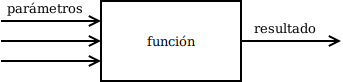
\includegraphics[width=0.5\textwidth]{graficos/funcion}
\end{center}
\end{figure}

Python viene equipado con muchas funciones, pero ya hemos dicho que, como
programadores, debíamos ser capaces de escribir nuevas instrucciones para la
computadora. Los programas de correo electrónico, navegación por Internet,
chat, juegos, escritura de textos o predicción de las condiciones
meteorológicas de los próximos días no son más que grandes programas
implementados introduciendo nuevas funciones a la máquina, escritas por uno o
muchos programadores.

Si queremos escribir una función (que llamaremos |holaMarta|) que devuelve la
cadena de texto ``Hola Marta! Estoy programando en Python.'', lo que debemos
hacer es ingresar el siguiente conjunto de líneas en Python:

\begin{lstlisting}[numbers=none]
>>> def holaMarta():
        return "Hola Marta! Estoy programando en Python."

>>>
\end{lstlisting}

|def holaMarta():| le indica a Python que estamos escribiendo una función cuyo
nombre es |holaMarta|, y los paréntesis indican que la función no recibe ningún
parámetro.  La instrucción |return <expresion>| indica cuál será el resultado
de la función.

La sangría\footnote{La sangría puede ingresarse utilizando dos o más espacios,
o presionando la tecla \keys{Tab}. Es importante prestar atención en no mezclar
espacios con tabs, para evitar ``confundir'' al intérprete.} con la que se
escribe la línea |return| es importante: le indica a Python que estamos
escribiendo el {\it cuerpo} de la función (es decir, las instrucciones que la
componen), que podría estar formado por más de una sentencia.  La línea en
blanco que dejamos luego de la instrucción |return| le indica a Python que
terminamos de escribir la función (y por eso aparece nuevamente el {\it
prompt}).

Si ahora queremos que la máquina ejecute la función |holaMarta|, debemos
escribir |holaMarta()| a continuación del cursor de Python:

\begin{lstlisting}[numbers=none]
>>> holaMarta()
'Hola Marta! Estoy programando en Python.'
>>>
\end{lstlisting}

Se dice que estamos {\it invocando} a la función |holaMarta|.  Al invocar una
función, se ejecutan las instrucciones que habíamos escrito en su cuerpo.

Nuestro amigo Pablo seguramente se pondrá celoso porque escribimos
una función que saluda a Marta, y nos pedirá que escribamos una
función que lo salude a él. Y así procederemos entonces:

\begin{lstlisting}[numbers=none]
>>> def holaPablo():
        return "Hola Pablo! Estoy programando en Python."
\end{lstlisting}

Pero, si para cada amigo que quiere que lo saludemos debemos que
escribir una función distinta, parecería que la computadora no es
una gran solución. A continuación veremos, sin embargo, que
podemos llegar a escribir una única función que se personalice en
cada invocación, para saludar a quien queramos. Para eso están
precisamente los parámetros.

Escribamos entonces una función |hola| que nos sirva para saludar a
cualquiera, de la siguiente manera:

\begin{lstlisting}[numbers=none]
>>> def hola(alguien):
        return "Hola " + alguien + "! Estoy programando en Python."
\end{lstlisting}

En este caso, además de indicar el nombre de la función (|hola|), debemos darle
un nombre al parámetro (|alguien|), cuyo valor será reemplazado por una cadena
de texto cuando se invoque a la función. Por ejemplo, podemos invocarla dos
veces, para saludar a Ana y a Juan:

\begin{lstlisting}[numbers=none]
>>> hola("Ana")
'Hola Ana! Estoy programando en Python.'
>>> hola("Juan")
'Hola Juan! Estoy programando en Python.'
\end{lstlisting}

\begin{problema}
\label{cuadrado}
Escribir una función que calcule el cuadrado de un número dado.
\end{problema}

\begin{solucion}
$ $\par
\begin{lstlisting}[numbers=none]
def cuadrado(n):
        return n * n
\end{lstlisting}

Para invocarla, deberemos hacer:
\begin{lstlisting}[numbers=none]
>>> cuadrado(5)
25
\end{lstlisting}
\end{solucion}

\begin{problema}
Piensa un número, duplícalo, súmale 6, divídelo por 2 y resta el número
que elegiste al comienzo. El número que queda es siempre 3.
\end{problema}

\begin{solucion}
Si bien es muy sencillo probar matemáticamente que el resultado de la secuencia
de operaciones será siempre 3 sin importar cuál sea el número elegido, podemos
aprovechar nuestros conocimientos de programación y probarlo empíricamente.

Para esto escribamos una función que reciba el número elegido y devuelva el
número que queda luego de efectuar las operaciones:

\begin{lstlisting}[numbers=none]
def f(elegido):
        return ((elegido * 2) + 6) / 2 - elegido
\end{lstlisting}

Tal vez el cuerpo de la función quedó poco entendible. Podemos mejorarlo
dividiendo la secuencia de operaciones en varias sentencias más pequeñas:

\begin{lstlisting}[numbers=none]
def f(elegido):
        n = elegido * 2
        n = n + 6
        n = n / 2
        n = n - elegido
        return n
\end{lstlisting}

Aquí utilizamos una variable llamada |n| y luego en cada sentencia vamos
reemplazando el valor de |n| por un valor nuevo.

Las dos soluciones que presentamos son equivalentes. Veamos si al invocar a |f|
con distintos números siempre devuelve 3 o no:

\begin{lstlisting}[numbers=none]
>>> f(9)
3.0
>>> f(4)
3.0
>>> f(118)
3.0
>>> f(165414606)
3.0
>>> f(0)
3.0
>>> f(-15)
3.0
\end{lstlisting}
\end{solucion}

\section{Una instrucción un poco más compleja: el ciclo definido}

\begin{problema}
Supongamos que queremos calcular la suma de los primeros 5 números cuadrados.

\begin{solucion}
Dado que ya tenemos la función |cuadrado|, podemos aprovecharla y hacer algo
como esto:

\begin{lstlisting}[numbers=none]
>>> def suma5Cuadrados():
        suma = 0
        suma = suma + cuadrado(1)
        suma = suma + cuadrado(2)
        suma = suma + cuadrado(3)
        suma = suma + cuadrado(4)
        suma = suma + cuadrado(5)
        return suma

>>> suma5Cuadrados()
55
\end{lstlisting}
\end{solucion}

Esto resuelve el problema, pero resulta poco satisfactorio. ¿Y si quisiéramos
encontrar la suma de los primeros 100 números cuadrados? En ese caso tendríamos
que repetir la línea |suma = suma + cuadrado(...)| 100 veces. ¿Se puede hacer
algo mejor que esto?

Para resolver este tipo de problema (repetir un cálculo para los valores
contenidos en un intervalo dado) de una manera más eficiente, introducimos el
concepto de {\it ciclo definido}, que tiene la siguiente forma:

\begin{lstlisting}[numbers=none]
for x in range(n1, n2):
        <hacer algo con x>
\end{lstlisting}

Esta instrucción se lee como:

\begin{itemize}
\item Generar la secuencia de valores enteros del intervalo $[n1, n2)$, y
\item Para cada uno de los valores enteros que toma |x| en el intervalo generado,
se debe hacer lo indicado por |<hacer algo con x>|.
\end{itemize}

La instrucción que describe el rango en el que va a realizar el ciclo
(|for x in range(...)|) es el {\it encabezado del ciclo}, y las instrucciones
que describen la acción que se repite componen el {\it cuerpo del ciclo}.
Todas las instrucciones que describen el cuerpo del ciclo deben tener una
sangría mayor que el encabezado del ciclo.

\begin{solucion}
Usemos un ciclo definido para resolver el problema anterior de manera más
compacta:

\begin{lstlisting}[numbers=none]
>>> def suma5Cuadrados():
        suma = 0
        for x in range(1, 6):
            suma = suma + cuadrado(x)
        return suma
\end{lstlisting}
\end{solucion}
\end{problema}

Notar que en nuestro ejemplo necesitamos recorrer todos los valores enteros
entre 1 y 5, y el rango generado por |range(n1, n2)| es {\it abierto} en |n2|.
Es decir, |x| tomará los valores |n1|, |n1 + 1|, |n1 + 2|, |...|, |n2 - 1|.
Por eso es que usamos |range(1, 6)|.

Incluso podemos hacer una función más genérica que permita calcular la suma de
los primeros |n| números cuadrados:

\begin{lstlisting}[numbers=none]
>>> def sumaCuadrados(n):
        suma = 0
        for x in range(1, n + 1):
            suma = suma + cuadrado(x)
        return suma

>>> sumaCuadrados(5)
55
>>> sumaCuadrados(100)
338350
\end{lstlisting}

\section{Construir programas y módulos}

El intérprete interactivo es muy útil para probar cosas, acceder a la ayuda,
inspeccionar el lenguaje, etc, pero tiene una gran limitación: ¡cuando cerramos
el intérprete perdemos todas las definiciones! Para conservar los programas que
vamos escribiendo, debemos escribir el código utilizando algún editor de texto,
y guardar el archivo con la extensión |.py|.

\begin{sabias_que}
El intérprete interactivo de python nos provee una ayuda en línea; es decir,
nos puede dar la documentación de cualquier función o instrucción. Para
obtenerla llamamos a la función |help()|. Si le pasamos por parámetro el nombre
de una función (por ejemplo |help(abs)| o |help(range)|) nos dará la
documentación de esa función. Para obtener la documentación de una instrucción
la debemos poner entre comillas; por ejemplo: |help('for')|, |help('return')|.
\end{sabias_que}

En el código \ref{cuad100.py} se muestra nuestro primer programa, |cuad100.py|,
que nos permite calcular la suma de los primeros 100 cuadrados.

\begin{codigo}{cuad100.py}{Imprime la suma de los primeros 100 números
    cuadrados}
\label{cuad100.py}
\begin{codigo-python}
def sumaCuadrados(n):
    suma = 0
    for x in range(1, n + 1):
        suma = suma + cuadrado(x)
    return suma

print("La suma de los primeros 100 cuadrados es", sumaCuadrados(100))
\end{codigo-python}
\end{codigo}

En la última línea del programa introducimos una función nueva: |print()|.
La función |print| recibe uno o más parámetros de cualquier tipo y los imprime
en la pantalla. ¿Por qué no habíamos utilizado |print| hasta ahora?

En el modo interactivo, Python imprime el resultado de cada expresión luego de
evaluarla:

\begin{lstlisting}[numbers=none]
>>> 2 + 2
4
\end{lstlisting}

En cambio, cuando Python ejecuta un programa |.py| no imprime absolutamente
nada en la pantalla, a menos que le indiquemos explícitamente que lo haga. Por
eso es que en |cuad100.py| debemos llamar a la función |print| para mostrar el
resultado.

Para ejecutar el programa debemos abrir una consola del sistema y ejecutar
|python cuad100.py|:

\begin{lstlisting}[language={},numbers=none]
$ python cuad100.py
La suma de los primeros 100 cuadrados es 338350
\end{lstlisting}

\section{Interacción con el usuario}

Ya vimos que la función |print| nos permite mostrar información al usuario del
programa. En algunos casos también necesitaremos que el usuario ingrese datos
al programa. Por ejemplo:

\begin{problema}
Escribir en Python un programa que pida al usuario que escriba su nombre, y
luego lo salude.

\begin{solucion}
Ya habíamos escrito la función |hola| que nos permitía saludar a una
persona si sabíamos su nombre. Pero aún no sabemos cómo obtener el nombre del
usuario. Para esto podemos usar la función |input|, como se muestra en el
Código \ref{saludar.py}.

\begin{codigo}{saludar.py}{Saluda al usuario posr su nombre}
\label{saludar.py}
\begin{codigo-python}
def hola(nombre):
    return "Hola " + nombre + "!"

def saludar():
    nombre = input("Por favor ingrese su nombre: ")
    saludo = hola(nombre)
    print(saludo)

saludar()
\end{codigo-python}
\end{codigo}
\end{solucion}
\end{problema}

En la función |saludar| usamos la función |input| para pedirle al usuario su
nombre. |input| presenta al usuario el mensaje que le pasamos por parámetro,
y luego le permite ingresar una cadena de texto. Cuando el usuario presiona la
tecla \keys{Enter}, |input| devuelve la cadena ingresada. Luego llamamos a
|hola| para generar el saludo, y a |print| para mostrarlo al usuario.

Para ejecutar el programa, nuevamente escribimos en la consola del sistema:

\begin{lstlisting}[language={},numbers=none]
$ python saludar.py
Por favor ingrese su nombre: Alan
Hola Alan!
\end{lstlisting}

\begin{problema}
Escribir en Python un programa que haga lo siguiente:

\begin{enumerate}
\item Muestra un mensaje de bienvenida por pantalla.
\item Le pide al usuario que introduzca dos números enteros $n1$ y $n2$.
\item Imprime el cuadrado de todos los números enteros del intervalo $[n1, n2)$.
\item Muestra un mensaje de despedida por pantalla.
\end{enumerate}
\end{problema}

\begin{solucion}
La solución a este problema se encuentra en el Código \ref{cuadrados.py}.

\begin{codigo}{cuadrados.py}{Imprime los cuadrados solicitados}
\label{cuadrados.py}
\begin{codigo-python}
def imprimir_cuadrados():
    print("Se calcularán cuadrados de números")

    n1 = int(input("Ingrese un número entero: "))
    n2 = int(input("Ingrese otro número entero: "))

    for x in range(n1, n2):
        print(x * x)

    print("Es todo por ahora")

imprimir_cuadrados()
\end{codigo-python}
\end{codigo}

Como siempre, podemos ejecutar el programa en la consola del sistema:

\begin{lstlisting}[language={},numbers=none]
$ python cuadrados.py
Se calcularán cuadrados de números
Ingrese un número entero: 5
Ingrese otro número entero: 8
25
36
49
Es todo por ahora
\end{lstlisting}
\end{solucion}

En el Código \ref{cuadrados.py} aparece una función que no habíamos
utilizado hasta ahora: |int|. ¿Por qué es necesario utilizar |int| para
resolver el problema?

En un programa Python podemos operar con cadenas de texto o con números.  Las
representaciones dentro de la computadora de un número y una cadena son muy
distintas. Por ejemplo, el número |12345678| se almacena en forma binaria y
típicamente ocupa 4 bytes, mientras que la cadena |"12345678"| es una sucesión
de caracteres en la que cada dígito se almacena de forma separada y ocupa (cada
uno) un byte.

La función |input| interpreta cualquier valor que el usuario ingresa mediante
el teclado como una cadena de caracteres. Es decir, |input| siempre devuelve
una cadena, incluso aunque el usuario haya ingresado una secuencia de dígitos.

Por eso es que introducimos la función |int|, que devuelve el parámetro que
recibe {\it convertido} a un número entero:

\begin{lstlisting}[numbers=none]
>>> int("42")
42
\end{lstlisting}

\begin{atencion}
Cuando introdujimos el concepto de función dijimos que una función recibe 0 o
más parámetros y devuelve un resultado. Pero en la función |saludar| que
escribimos en el Código \ref{saludar.py} no hay ninguna instrucción
|return|\ldots
es decir, |saludar| es una función que no recibe parámetros {\it ¡y no devuelve
nada!}.

Esto es perfectamente válido: no necesitamos que |saludar| reciba parámetros
porque estamos utilizando la función |input| para obtener la entrada del
usuario, y no necesitamos que la función devuelva nada, porque su único
cometido es {\it imprimir} un mensaje en la pantalla.

Cuando decimos que las funciones {\it reciben} datos a través de los parámetros
y {\it devuelven} datos mediante la instrucción |return|, las funciones |input|
y |print| son dos notables excepciones a esta regla. |input| permite que una
función reciba información mediante la entrada del usuario, y |print| permite
que una función muestre información al usuario.

\begin{center}
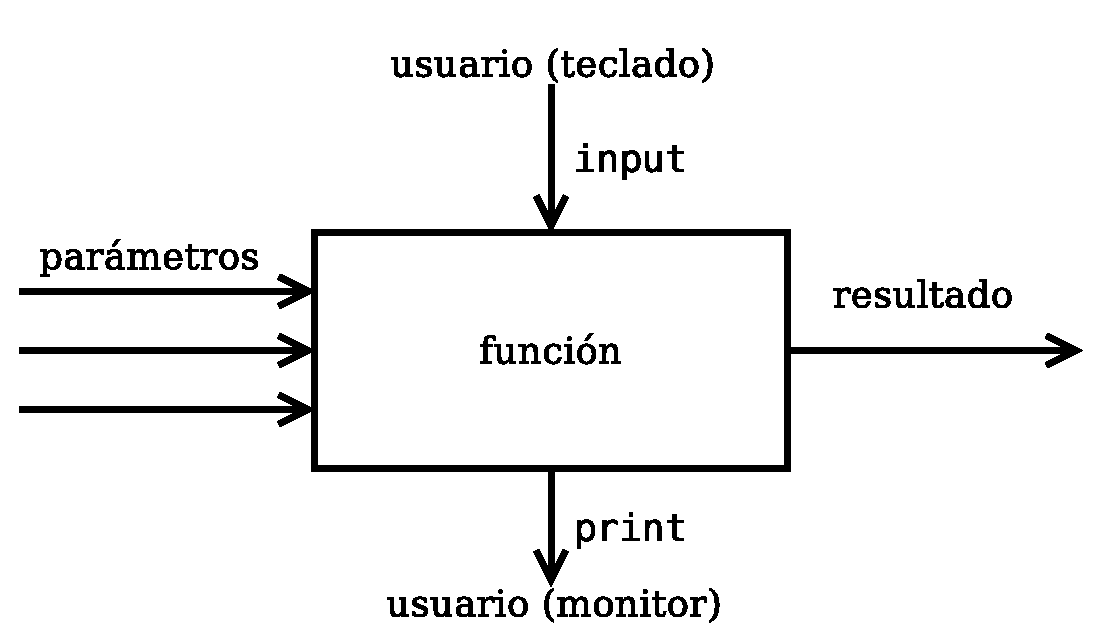
\includegraphics[width=0.5\textwidth]{graficos/funcion_input_print}
\end{center}

Si una función devuelve información mediante |return|, esa información la
podemos reutilizar: por ejemplo, la podemos guardar en una variable, o pasarla
a otra función en algunos de sus parámetros. En cambio, si una función
usa |print|, no será posible reutilizar la información que se imprimió en la
pantalla. De la misma manera, una función que recibe información mediante
parámetros es mucho más reutilizable que una función que usa |input|.

Por eso es buena práctica de programación limitar el uso de |input| y |print|
al mínimo indispensable: utilizar |input| únicamente en los lugares donde
necesitamos que el usuario ingrese datos, y |print| únicamente donde
necesitamos mostrar información al usuario.
\end{atencion}

%
% Lenguajes optimistas vs controladores
%
\clearpage

\section{Estado y computación}

A lo largo de la ejecución de un programa las variables pueden
cambiar el valor con el que están asociadas. En un momento dado
uno puede detenerse a observar a qué valor se refiere cada una de
las variables del programa. Esa ``foto'' que indica en un momento dado
a qué valor hace referencia cada una de las variables se denomina
{\it estado}. También hablaremos del {\it estado de una variable}
para indicar a qué valor está asociada esa variable, y usaremos la
notación |n| $\ra$ 13 para describir el estado de la variable |n| (e indicar
que está asociada al número 13).

A medida que las variables cambian de valores a los que se
refieren, el programa va cambiando de estado. La sucesión de todos
los estados por los que pasa el programa en una ejecución dada se
denomina {\it computación}.

Para ejemplificar estos conceptos veamos qué sucede cuando se
ejecuta el programa |cuadrados.py|:

\begin{longtable}[c]{|p{5.5cm}|p{5.5cm}|p{1.5cm}|}
\hline
{\bf Instrucción} & {\bf Qué sucede} & {\bf Estado}\\

\hline
\lstinline!print("Se calcularán!
\lstinline!cuadrados de números")!
&
Se despliega el texto ``Se calcularán cuadrados de
números'' en la pantalla.
&
\\

\hline
\lstinline!n1 = int(input("Ingrese !
\lstinline!un número entero: "))!
&
Se despliega el texto ``Ingrese un número entero: '' en la pantalla y el
programa se queda esperando que el usuario ingrese un número.
&
\\

\hline
&
Supondremos que el usuario ingresa el número 3
y luego oprime la tecla \keys{Enter}.

Se asocia el número 3 con la variable \lstinline!n1!.
&
\lstinline!n1! $\ra$ 3\\

\hline
\lstinline!n2 = int(input("Ingrese !
\lstinline!otro número entero: "))!
&
Se despliega el texto ``Ingrese otro número entero:'' en la
pantalla y el programa se queda esperando que el
usuario ingrese un número.
&
\lstinline!n1! $\ra$ 3\\

\hline
&
Supondremos que el usuario ingresa el número 5
y luego oprime la tecla \keys{Enter}.

Se asocia el número 5 con la variable \lstinline!n2!.
&
\lstinline!n1! $\ra$ 3 \newline
\lstinline!n2! $\ra$ 5 \\

\hline
\lstinline+for x in range(n1, n2):+
&
Se asocia el primer número de \lstinline![n1,n2)! con la variable
\lstinline!x! y se ejecuta el cuerpo del ciclo.
&
\lstinline!n1! $\ra$ 3 \newline
\lstinline!n2! $\ra$ 5 \newline
\lstinline!x! $\ra$ 3 \\

\hline
\lstinline+    print(x * x)+
&
Se imprime por pantalla el valor de \lstinline!x! * \lstinline!x! (9)
&
\lstinline!n1! $\ra$ 3 \newline
\lstinline!n2! $\ra$ 5 \newline
\lstinline!x! $\ra$ 3 \\

\hline
\lstinline+for x in range(n1, n2):+
&
Se asocia el segundo número de \lstinline![n1,n2)! con la variable
\lstinline!x! y se ejecuta el cuerpo del ciclo.
&
\lstinline!n1! $\ra$ 3 \newline
\lstinline!n2! $\ra$ 5 \newline
\lstinline!x! $\ra$ 4 \\

\hline
\lstinline+    print(x*x)+
&
Se imprime por pantalla el valor de \lstinline!x! * \lstinline!x! (16)
&
\lstinline!n1! $\ra$ 3 \newline
\lstinline!n2! $\ra$ 5 \newline
\lstinline!x! $\ra$ 4 \\

\hline
\lstinline+for x in range(n1, n2):+
&
Como no quedan más valores por tratar en \lstinline![n1, n2)!,
se sale del ciclo.
&
\lstinline!n1! $\ra$ 3 \newline
\lstinline!n2! $\ra$ 5 \newline
\lstinline!x! $\ra$ 4 \\

\hline
\lstinline+print("Es todo por ahora")+
&
Se despliega por pantalla el mensaje ``Es todo por ahora''
&
\lstinline!n1! $\ra$ 3 \newline
\lstinline!n2! $\ra$ 5 \newline
\lstinline!x! $\ra$ 4 \\

\hline
\end{longtable}

\subsection{Depuración de programas}

Una manera de seguir la evolución del estado es insertar instrucciones de impresión
en sitios críticos del programa. Esto nos será de utilidad para detectar errores
y también para comprender cómo funcionan determinadas instrucciones.

Por ejemplo, podemos insertar llamadas a la función |print| en el Código
\ref{cuadrados.py} para inspeccionar el contenido de las variables:

\begin{lstlisting}[numbers=none]
def imprimir_cuadrados():
    print("Se calcularán cuadrados de números")

    n1 = int(input("Ingrese un número entero: "))
    print("el valor de n1 es:", n1)
    n2 = int(input("Ingrese otro número entero: "))
    print("el valor de n2 es:", n2)

    for x in range(n1, n2):
        print("el valor de x es:", x)
        print(x * x)

    print("Es todo por ahora")

imprimir_cuadrados()
\end{lstlisting}

En este caso, la salida del programa será:

\begin{lstlisting}[language={},numbers=none]
$ python cuadrados.py
Se calcularán cuadrados de números
Ingrese un número entero: 5
el valor de n1 es: 5
Ingrese otro número entero: 8
el valor de n2 es: 8
el valor de x es: 5
25
el valor de x es: 6
36
el valor de x es: 7
49
Es todo por ahora
\end{lstlisting}

Si utilizamos este método para depurar el programa, tendremos que recordar
eliminar las llamadas |print| una vez que terminemos.

\newpage
\section{Ejercicios}

\begin{ejercicio}
Correr tres veces el programa \lstinline!cuadrados.py! con valores
de entrada (3,5), (3,3) y (5,3) respectivamente. ¿Qué sucede en
cada caso?
\end{ejercicio}

\begin{ejercicio}
La salida del programa \lstinline!cuadrados.py! es poco
informativa. Modificar el programa para que ponga el
número junto a su cuadrado.
\end{ejercicio}

\extractionlabel{guia}
\begin{ejercicio}
Escribir un programa que pregunte al usuario:
\begin{partes}
  \item su nombre, y luego lo salude.
  \item dos números, y luego muestre el producto.
\end{partes}
\end{ejercicio}

\extractionlabel{guia}
\begin{ejercicio} Implementar algoritmos que permitan:
\begin{partes}
 \item Calcular el perímetro de un rectángulo dada su base y su altura.
 \item Calcular el área de un rectángulo dada su base y su altura.
 \item Calcular el área de un rectángulo (alineado con los ejes $x$ e $y$)
     dadas sus coordenadas $x1$, $x2$, $y1$, $y2$.
 \item Calcular el perímetro de un círculo dado su radio.
 \item Calcular el área de un círculo dado su radio.
 \item Calcular el volumen de una esfera dado su radio.
 \item Dados los catetos de un triángulo rectángulo, calcular su hipotenusa.
\end{partes}
\end{ejercicio}

\extractionlabel{guia}
\begin{ejercicio}
Mostrar el resultado de ejecutar estos bloques de código en el
intérprete de python:
\begin{partes}
\item \begin{verbatim}
>>> for i in range(5):
        print(i * i)
\end{verbatim}
\item \begin{verbatim}
>>> for i in range(2, 6):
        print(i, 2 ** i)
\end{verbatim}
\end{partes}
\end{ejercicio}

\extractionlabel{guia}
\begin{ejercicio} Implementar un algoritmo que, dado un número entero $n$,
    permita calcular su factorial.
\end{ejercicio}

\extractionlabel{guia}
\begin{ejercicio} Implementar algoritmos que resuelvan los siguientes
problemas:
\begin{partes}
  \item Dados dos números, imprimir la suma, resta, división y multiplicación
  de ambos.
  \item Dado un número entero $n$, imprimir su tabla de multiplicar.
\end{partes}
\end{ejercicio}

\extractionlabel{guia}
\begin{ejercicio}
Escribir un programa que le pida una palabra al usuario, para luego
imprimirla 1000 veces, en una única línea, con espacios intermedios.

{\it Ayuda:} Investigar acerca del parámetro |end| de la función |print|.
\end{ejercicio}
